\documentclass{article}

\usepackage{amsmath,amssymb,amsthm,graphicx,subfigure}

\pagestyle{myheadings}

\pdfpagewidth 8.5in
\pdfpageheight 11 in

\setlength\topmargin{0in}
\setlength\textheight{8.5in}
\setlength\textwidth{6.5in}
\setlength\oddsidemargin{0in}
\setlength\evensidemargin{0in}

\newcommand{\suchthat}{\ni}
\newcommand{\onlyif}{\Longleftrighttriangle}
\newcommand{\definedby}{\triangleq}
\newcommand{\union}{\bigcup}
\newcommand{\intersect}{\bigcap}
\newcommand{\where}{\mid}
\newcommand{\inverse}{\overline}

\title{CIT 596 Homework 3}
\author{Steven Tomcavage\\stomcava@seas.upenn.edu}
\date{February 17, 2011}

\markboth{\hfill Steven Tomcavage }{\hfill Steven Tomcavage }

\begin{document}

\maketitle

\section{Exercise 1.13}

Give a DFA that recognizes the language $F$ where $F$ is the language of all
strings over $\{0, 1\}$ that do not contain a pair of $1$s which are separated
by an odd number of symbols.

\begin{figure}[h!]
	\centering
	\subfigure[The NFA $A$ accepts $\inverse{F}$] {
		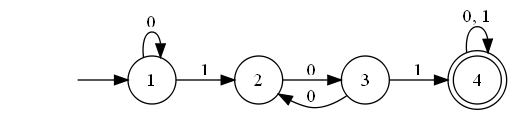
\includegraphics[height=0.75in]{1_13_a.png}
	}
	\subfigure[The DFA $B$ accepts $F$] 
	{
		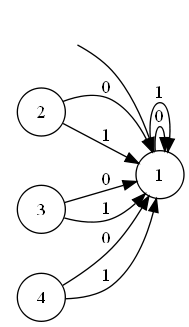
\includegraphics[height=0.75in]{1_13_b.png}
	}
	\caption{DFA for Exercise 1.13}
\end{figure}

\section{Exercise 1.16b}

Convert the given NFA (omitted) to a DFA. 

\begin{figure}[h!]
	\centering
	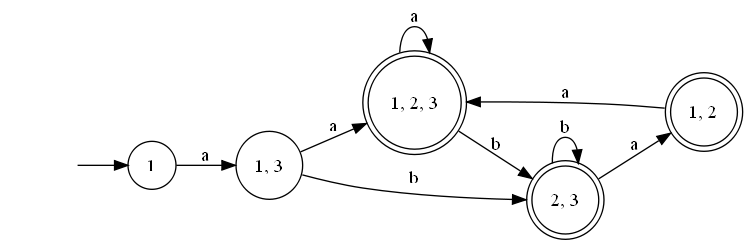
\includegraphics[height=1.5in]{1_16.png}
	\caption{DFA for Exercise 1.16b}
\end{figure}

\section{Exercise 1.17a}

Give an NFA recognizing the language $(01 \union 001 \union 010)^\star$.

\begin{figure}[h!]
	\centering
	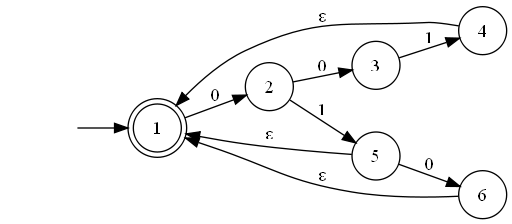
\includegraphics[height=1.5in]{1_17_a.png}
	\caption{DFA for Exercise 1.17a}
\end{figure}

\section{Exercise 1.17b}

Convert the NFA from Exercise 1.17a to an equivalent DFA.

\begin{figure}[h!]
	\centering
	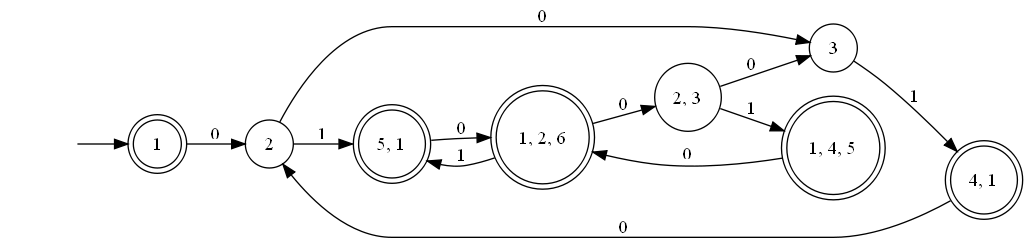
\includegraphics[height=1.25in]{1_17_b.png}
	\caption{DFA for Exercise 1.17b}
\end{figure}

\section{Exercise 1.19b}

Convert the following regular expression to an NFA: $(((00)^\star (11)) \union
01)^\star$.

\begin{figure}[h!]
	\centering
	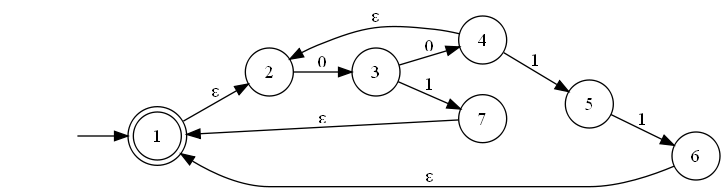
\includegraphics[height=1.25in]{1_19.png}
	\caption{DFA for Exercise 1.19b}
\end{figure}

\section{Exercise 1.21b}

Convert the following NFA to a regular expression.

\begin{figure}[h!]
	\centering
	\subfigure[The original NFA.] {
		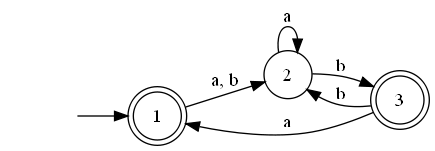
\includegraphics[height=1.0in]{1_21_a.png}
	}
	\subfigure[Add a start and end state.] {
		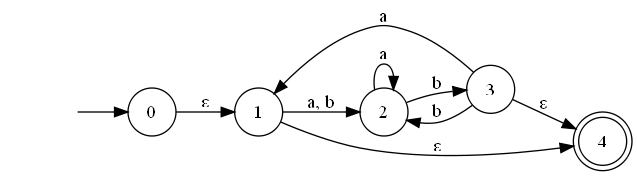
\includegraphics[height=1.0in]{1_21_b.png}
	}
	\subfigure[Rip out state 2.] {
		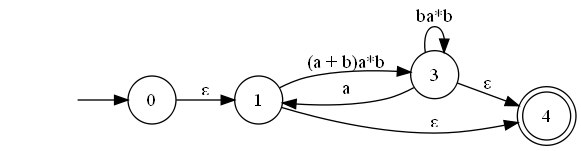
\includegraphics[height=1.0in]{1_21_c.png}
	}
	\subfigure[Rip out state 3.] {
		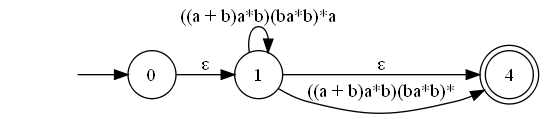
\includegraphics[height=0.75in]{1_21_d.png}
	}
	\subfigure[Rip out state 1 to get the final regular expression.] {
		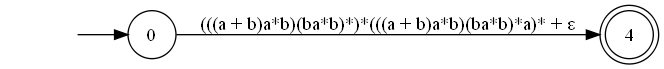
\includegraphics[height=0.5in]{1_21_e.png}
	}
	\caption{DFA for Exercise 1.21b}
\end{figure}

\newpage

\section{Exercise 1.28c}

Convert the regular expression $(a \union b^+) a^+ b^+$ to an NFA, given that
$\Sigma = \{a, b\}$.

\begin{figure}[h!]
	\centering
	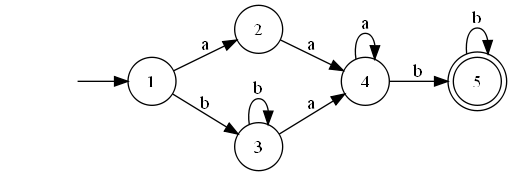
\includegraphics[height=1.5in]{1_28.png}
	\caption{DFA for Exercise 1.28c}
\end{figure}

\section{Exercie 1.29b}

Use the pumping lemma to show that the language $A_2 = \{ www \where w \in
\{a, b\}^\star \}$ is not regular.

\begin{proof}
	\mbox{}
	\begin{enumerate}
	  \item Assume $A_2$ is regular.
	  \item Let the three $w$s in the language be represented as $w_1, w_2, w_3$.
	  \item Then $|w_1| = |w_2| = |w_3|$.
	  \item Let $xyz = w_1$.
	  \item Given that $y \ne \epsilon$ and either $x$ or $z \ne \epsilon$, then
	  $y < w_2$ and $y < w_3$.
	  \item Pumping $y$ up will make $|w_1| \ne |w_2|$, which breaks the language.
	  \item Therefore, since the langauge $A_2$ cannot be pumped, is not regular.
	  \qedhere
	\end{enumerate}
\end{proof}

\section{Exercie 1.32}

Show that the language $B$ (omitted) is regular.

\begin{proof}
	\mbox{}
	\begin{enumerate}
	  \item Let $B_R$ be the reverse language of $B$.
	  \item Given that a regular language can be pumped, and that the reverse of a
	  regular language is also a regular language, $B_R$ should be pumpable if $B$
	  is a regular language.
	  \item Let $b_1$ be the top row of $B_R$, $b_2$ be the middle row, and $b_3$
	  be the bottom, or sum, row. 
	  \item Since $b_3$ is a summation of $b_1$, $b_2$, there must be a carry bit
	  which works its way from left to right through $B_R$ (since $B_R$ is a
	  reverse of the summation $B$).
	  \item Let $w = xyz$ be some section of $B_R$, where $y$ is the section being
	  pumped.
	  \item Let $j$ be the carry-in bit comming in to $y$ and $k$ be the carry-out
	  bit comming out of $y$.
	  \item If $j = k$ then the summation $b_3$ would still be correct after
	  pumping and $y$ can be pumped.
	  \item If $j \ne k$, then I'm not sure what to do to make $y$ pumpable, so
	  I'll just say something goes here to prove that $B_R$ can be pumped when $j \ne
	  k$.
	  \item Since $B_R$ can be pumped in all cases, then $B_R$ is a regular
	  language.
	  \item Therefore, since $B_R$ is a regular language, than $B$ is a regular
	  language. \qedhere
	\end{enumerate}
\end{proof}

\section{Exercise 1.51}

If $x$ and $y$ are indistinguishable by $L$, show that their
indistinguishability is an equivalence relation.

I looked up equivalence relations and found that they have to do with set
theory. When I took CIT592, we had only the briefest glance into set theory. I'm not
sure I know how to prove this, or even where to start with proofs about sets, so
I'm skipping it.

\section{Exercise 1.53}

Let $\Sigma = \{0, 1, +, =\}$ and $ADD = \{ x=y+z \where x, y, z \text{ are
binary integers and } x \text{ is the sum of } y \text{ and } z\}$. Show that
the language $ADD$ is not regular.

\begin{proof}
	\mbox{}
	\begin{enumerate}
	  \item Assume that $ADD$ is regular.
	  \item Let $p$ be the pumping length of $ADD$.
	  \item Let $w = ADD = x_1 y_1 z_1$, where $0 > y_1 \leq p$.
	  \item Since the symbols $=$ and $+$ cannot be pumped, the only pumpable
	  segments must be the binary representation of integers in $x$, $y$, and $z$.
	  \item If we assume that $x_1 = \epsilon$, then $z_1 \ne \epsilon$ and $y_1$
	  must either be $x$ or $x=y$. Pumping either one would change the equality
	  of the summation and break the language.
	  \item If we assume that $z_1 = \epsilon$, then $x_1 \ne \epsilon$ and $y_1$
	  must either be $y+z$ or $z$. Again, pumping either one would change the
	  equality of the summation and break the language.
  	  \item Therefore, since the langauge $ADD$ cannot be pumped, is not regular.
  	  \qedhere
	\end{enumerate}
\end{proof}

\section{Exercise 1.55c}

What is the minimum pumping length for $001 \union 0^\star1^\star$?

The minimum pumping length is 2 because at that length, either a 0 or a 1
in the second position could be pumped. 

\section{Exercise 1.55h}

What is the minimum pumping length for $10(11^\star0)^\star0$?

The minimum pumping length is 5, where the string 10100 can be divided as $x
= 10, y = 1, z = 00$.

\end{document}
